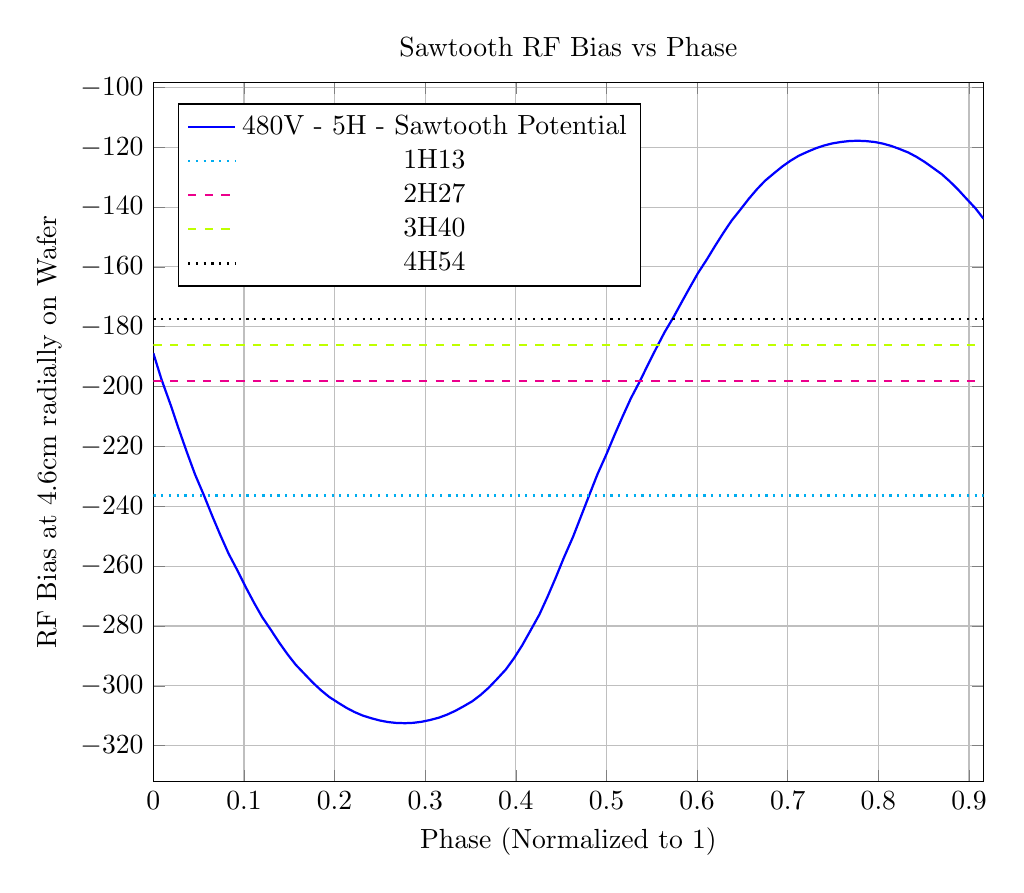
\begin{tikzpicture}
\begin{axis}[
    width=\textwidth,
    xlabel={Phase (Normalized to 1)},
    xmin=0,
    xmax=0.916,
    ylabel={RF Bias at 4.6cm radially on Wafer},
    title={Sawtooth RF Bias vs Phase},
    legend pos=north west,
    grid=major,
    legend style={fill=white, draw=black},
    legend entries={480V - 5H - Sawtooth Potential, 1H13, 2H27, 3H40, 4H54},
]
    \addplot[thick, blue] coordinates {(0.000, -188.800) (0.009, -197.569) (0.019, -206.005) (0.028, -214.109) (0.037, -221.881) (0.046, -229.321) (0.056, -236.430) (0.065, -243.209) (0.074, -249.657) (0.083, -255.776) (0.093, -261.565) (0.102, -267.025) (0.111, -272.157) (0.120, -276.961) (0.130, -281.438) (0.139, -285.587) (0.148, -289.410) (0.157, -292.907) (0.167, -296.078) (0.176, -298.926) (0.185, -301.463) (0.194, -303.701) (0.204, -305.653) (0.213, -307.334) (0.222, -308.754) (0.231, -309.928) (0.241, -310.868) (0.250, -311.588) (0.259, -312.098) (0.268, -312.397) (0.278, -312.484) (0.287, -312.356) (0.296, -312.009) (0.305, -311.442) (0.315, -310.651) (0.324, -309.633) (0.333, -308.387) (0.342, -306.901) (0.352, -305.142) (0.361, -303.066) (0.370, -300.631) (0.379, -297.795) (0.389, -294.516) (0.398, -290.752) (0.407, -286.459) (0.416, -281.598) (0.426, -276.150) (0.435, -270.195) (0.444, -263.830) (0.453, -257.154) (0.463, -250.266) (0.472, -243.264) (0.481, -236.247) (0.490, -229.313) (0.500, -222.560) (0.509, -216.070) (0.518, -209.843) (0.527, -203.857) (0.537, -198.089) (0.546, -192.517) (0.555, -187.119) (0.564, -181.874) (0.574, -176.757) (0.583, -171.749) (0.592, -166.834) (0.601, -162.032) (0.611, -157.374) (0.620, -152.887) (0.629, -148.601) (0.638, -144.544) (0.648, -140.746) (0.657, -137.235) (0.666, -134.040) (0.675, -131.183) (0.685, -128.654) (0.694, -126.436) (0.703, -124.513) (0.712, -122.868) (0.722, -121.484) (0.731, -120.345) (0.740, -119.434) (0.749, -118.735) (0.759, -118.234) (0.768, -117.931) (0.777, -117.831) (0.786, -117.939) (0.796, -118.260) (0.805, -118.797) (0.814, -119.557) (0.823, -120.543) (0.833, -121.761) (0.842, -123.214) (0.851, -124.908) (0.860, -126.848) (0.870, -129.037) (0.879, -131.481) (0.888, -134.185) (0.897, -137.153) (0.907, -140.390) (0.916, -143.900)};
    \addplot[dotted, thick, cyan] coordinates {(0.000, -236.400) (0.020, -236.400) (0.041, -236.400) (0.061, -236.400) (0.082, -236.400) (0.102, -236.400) (0.122, -236.400) (0.143, -236.400) (0.163, -236.400) (0.184, -236.400) (0.204, -236.400) (0.224, -236.400) (0.245, -236.400) (0.265, -236.400) (0.286, -236.400) (0.306, -236.400) (0.327, -236.400) (0.347, -236.400) (0.367, -236.400) (0.388, -236.400) (0.408, -236.400) (0.429, -236.400) (0.449, -236.400) (0.469, -236.400) (0.490, -236.400) (0.510, -236.400) (0.531, -236.400) (0.551, -236.400) (0.571, -236.400) (0.592, -236.400) (0.612, -236.400) (0.633, -236.400) (0.653, -236.400) (0.673, -236.400) (0.694, -236.400) (0.714, -236.400) (0.735, -236.400) (0.755, -236.400) (0.776, -236.400) (0.796, -236.400) (0.816, -236.400) (0.837, -236.400) (0.857, -236.400) (0.878, -236.400) (0.898, -236.400) (0.918, -236.400) (0.939, -236.400) (0.959, -236.400) (0.980, -236.400) (1.000, -236.400)};
    \addplot[dashed, thick, magenta] coordinates {(0.000, -198.200) (0.020, -198.200) (0.041, -198.200) (0.061, -198.200) (0.082, -198.200) (0.102, -198.200) (0.122, -198.200) (0.143, -198.200) (0.163, -198.200) (0.184, -198.200) (0.204, -198.200) (0.224, -198.200) (0.245, -198.200) (0.265, -198.200) (0.286, -198.200) (0.306, -198.200) (0.327, -198.200) (0.347, -198.200) (0.367, -198.200) (0.388, -198.200) (0.408, -198.200) (0.429, -198.200) (0.449, -198.200) (0.469, -198.200) (0.490, -198.200) (0.510, -198.200) (0.531, -198.200) (0.551, -198.200) (0.571, -198.200) (0.592, -198.200) (0.612, -198.200) (0.633, -198.200) (0.653, -198.200) (0.673, -198.200) (0.694, -198.200) (0.714, -198.200) (0.735, -198.200) (0.755, -198.200) (0.776, -198.200) (0.796, -198.200) (0.816, -198.200) (0.837, -198.200) (0.857, -198.200) (0.878, -198.200) (0.898, -198.200) (0.918, -198.200) (0.939, -198.200) (0.959, -198.200) (0.980, -198.200) (1.000, -198.200)};
    \addplot[dashed, thick, lime] coordinates {(0.000, -186.000) (0.020, -186.000) (0.041, -186.000) (0.061, -186.000) (0.082, -186.000) (0.102, -186.000) (0.122, -186.000) (0.143, -186.000) (0.163, -186.000) (0.184, -186.000) (0.204, -186.000) (0.224, -186.000) (0.245, -186.000) (0.265, -186.000) (0.286, -186.000) (0.306, -186.000) (0.327, -186.000) (0.347, -186.000) (0.367, -186.000) (0.388, -186.000) (0.408, -186.000) (0.429, -186.000) (0.449, -186.000) (0.469, -186.000) (0.490, -186.000) (0.510, -186.000) (0.531, -186.000) (0.551, -186.000) (0.571, -186.000) (0.592, -186.000) (0.612, -186.000) (0.633, -186.000) (0.653, -186.000) (0.673, -186.000) (0.694, -186.000) (0.714, -186.000) (0.735, -186.000) (0.755, -186.000) (0.776, -186.000) (0.796, -186.000) (0.816, -186.000) (0.837, -186.000) (0.857, -186.000) (0.878, -186.000) (0.898, -186.000) (0.918, -186.000) (0.939, -186.000) (0.959, -186.000) (0.980, -186.000) (1.000, -186.000)};
    \addplot[dotted, thick, black] coordinates {(0.000, -177.300) (0.020, -177.300) (0.041, -177.300) (0.061, -177.300) (0.082, -177.300) (0.102, -177.300) (0.122, -177.300) (0.143, -177.300) (0.163, -177.300) (0.184, -177.300) (0.204, -177.300) (0.224, -177.300) (0.245, -177.300) (0.265, -177.300) (0.286, -177.300) (0.306, -177.300) (0.327, -177.300) (0.347, -177.300) (0.367, -177.300) (0.388, -177.300) (0.408, -177.300) (0.429, -177.300) (0.449, -177.300) (0.469, -177.300) (0.490, -177.300) (0.510, -177.300) (0.531, -177.300) (0.551, -177.300) (0.571, -177.300) (0.592, -177.300) (0.612, -177.300) (0.633, -177.300) (0.653, -177.300) (0.673, -177.300) (0.694, -177.300) (0.714, -177.300) (0.735, -177.300) (0.755, -177.300) (0.776, -177.300) (0.796, -177.300) (0.816, -177.300) (0.837, -177.300) (0.857, -177.300) (0.878, -177.300) (0.898, -177.300) (0.918, -177.300) (0.939, -177.300) (0.959, -177.300) (0.980, -177.300) (1.000, -177.300)};
\end{axis}
\end{tikzpicture}